\documentclass[tikz,border=12pt]{standalone}
\usepackage{amsmath}
\usepackage[T1]{fontenc}
\usepackage{tikz}
\usetikzlibrary{positioning,arrows.meta,backgrounds,fit,calc,decorations.pathreplacing}

\definecolor{cgray}{RGB}{120,120,120}
\definecolor{cblue}{RGB}{56,110,190}
\definecolor{cbluefill}{RGB}{205,225,248}
\definecolor{cgreen}{RGB}{70,150,70}
\definecolor{cgreenfill}{RGB}{214,238,210}
\definecolor{cpurple}{RGB}{130,90,200}
\definecolor{cpurplefill}{RGB}{226,214,246}
\definecolor{corange}{RGB}{225,140,45}
\definecolor{corangefill}{RGB}{252,228,193}
\definecolor{cnavy}{RGB}{20,40,80}

% tapered volume: fill draw xFront yc hBack hFront nplanes gap
\newcommand{\voltap}[8]{%
  \foreach \k in {1,...,#7}{%
    \pgfmathsetmacro{\xx}{#3-(#7-\k)*#8}%
    \pgfmathsetmacro{\hh}{#5+(#6-#5)*(\k-1)/(#7-1)}%
    \fill[#1,draw=#2,line width=0.5pt]
      (\xx,{#4-\hh/2})--++(0.5,0.28)--++(0,\hh)--++(-0.5,-0.28)--cycle;}}
% x yc
\newcommand{\imgblock}[2]{%
\begin{scope}[shift={(#1,{#2-1.21})}]
  \foreach \i in {0,...,6}{
    \draw[cgray!55,line width=0.3pt] ({\i*0.2},{\i*0.12})--++(0,1.7);
    \draw[cgray!55,line width=0.3pt] (0,{\i*0.24})--++(1.2,0.72);}
  \draw[cgray,line width=0.8pt] (0,0)--(1.2,0.72)--(1.2,2.42)--(0,1.7)--cycle;
\end{scope}}
% x yc
\newcommand{\actbox}[2]{%
  \node[draw=cgreen,fill=cgreenfill,rounded corners=2pt,minimum width=0.9cm,
        minimum height=0.9cm,line width=0.7pt] at (#1,#2){};
  \draw[cgreen!75!black,line width=0.9pt]
    (#1-0.29,{#2-0.23})..controls (#1-0.04,{#2-0.23}) and (#1+0.04,{#2+0.23})..(#1+0.29,{#2+0.23});}
% x yc h
\newcommand{\latentcol}[3]{%
  \fill[cpurplefill,draw=cpurple,line width=0.6pt]
    (#1,{#2-#3/2})--++(0.5,0.28)--++(0,#3)--++(-0.5,-0.28)--cycle;
  \foreach \t in {1,2,3}{\pgfmathsetmacro{\yy}{#2-#3/2+\t*#3/4}
    \draw[cpurple!55,line width=0.3pt] (#1,\yy)--++(0.5,0.28);}}

\begin{document}
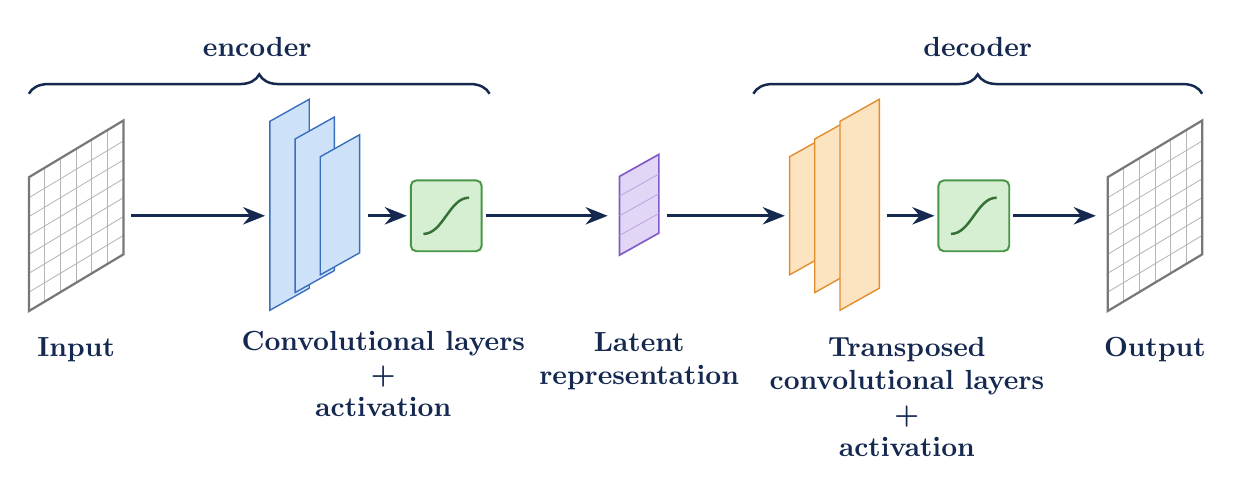
\begin{tikzpicture}[
  font=\footnotesize,
  >={Stealth[length=2.8mm,width=2.2mm]},
]
\def\y{0}

% ===== INPUT =====
\imgblock{0.3}{\y}
\node[cnavy,font=\bfseries] at (0.9,-1.7) {Input};
\draw[cnavy,->,line width=1.0pt] (1.6,\y)--(3.3,\y);

% ===== CONV LAYERS + ACTIVATION (tapering down) =====
\voltap{cbluefill}{cblue}{4.0}{\y}{2.4}{1.5}{3}{0.32}
\actbox{5.6}{\y}
\node[cnavy,font=\bfseries,align=center] at (4.8,-2.01) {Convolutional layers\\+ \\activation};
\draw[cnavy,->,line width=1.0pt] (4.6,\y)--(5.1,\y);
\draw[cnavy,->,line width=1.0pt] (6.1,\y)--(7.65,\y);

% ===== LATENT (bottleneck) =====
\latentcol{7.8}{\y}{1.0}
\node[cnavy,font=\bfseries,align=center] at (8.05,-1.85) {Latent\\representation};
\draw[cnavy,->,line width=1.0pt] (8.4,\y)--(9.9,\y);

% ===== TRANSPOSED CONV LAYERS + ACTIVATION (tapering up) =====
\voltap{corangefill}{corange}{10.6}{\y}{1.5}{2.4}{3}{0.32}
\actbox{12.3}{\y}
\node[cnavy,font=\bfseries,align=center] at (11.45,-2.3) {Transposed\\ convolutional layers \\+ \\activation};
\draw[cnavy,->,line width=1.0pt] (11.2,\y)--(11.8,\y);
\draw[cnavy,->,line width=1.0pt] (12.8,\y)--(13.85,\y);

% ===== OUTPUT =====
\imgblock{14.0}{\y}
\node[cnavy,font=\bfseries] at (14.6,-1.7) {Output};

% ===== braces =====
\draw[cnavy,line width=0.9pt,decorate,decoration={brace,amplitude=7pt}]
  (0.3,1.55)--(6.15,1.55);
\node[cnavy,font=\bfseries] at (3.2,2.15) {encoder};
\draw[cnavy,line width=0.9pt,decorate,decoration={brace,amplitude=7pt}]
  (9.5,1.55)--(15.2,1.55);
\node[cnavy,font=\bfseries] at (12.35,2.15) {decoder};

\end{tikzpicture}
\end{document}
